\documentclass[12pt,a4paper]{article}
\usepackage[a4paper,top=1.5cm, bottom=1.5cm, left=1.5cm, right=1.5cm]{geometry}
\usepackage[T2A]{fontenc}
\usepackage[utf8]{inputenc}
\usepackage[russian]{babel}
\usepackage{amsmath}
\usepackage{amssymb}
\usepackage{graphicx}
\usepackage{floatrow}
\usepackage{booktabs}
\usepackage{wrapfig}
\usepackage{lipsum}
\usepackage{subcaption}
\usepackage{float}
\restylefloat{table}

\newcommand{\figref}[1]{(См. рис. \ref{#1})}
\newcommand{\e}[1]{\text{$\cdot10^{#1}$}}

\title{Лабораторная работа 2.2.3\\ Измерение теплопроводности воздуха при атмосферном давлении}
\author{Симанкович Александр \\ Б01-104}
\date{30.03.2022}


\begin{document}
	\maketitle
	
	\section*{Цель работы}
		
	$\quad$ Измерить коэффициент теплопроводности воздуха при атмосферном давлении в зависимости от температуры.
	
	\section*{Оборудование и приборы} 
	$\quad$ Цилиндрическая колба с натянутой по оси нитью;
	термостат; 
	вольтметр и амперметр (цифровые мультиметры); 
	эталонное сопротивление; источник постоянного напряжения; 
	реостат (или магазин сопротивлений).
	
	\section*{Теоретическое введение}
	
	$\quad$ Теплопроводность — это процесс передачи тепловой энергии от нагретых частей системы к холодным за счёт хаотического движения частиц среды(молекул, атомов и т.п.).
	В газах теплопроводность осуществляется за счёт непосредственной передачи кинетической энергии от быстрых молекул к медленным при их столкновениях. 
	Перенос тепла описывается законом Фурье, утверждающим, что плотность потока энергии $\vec{q} \: [\frac{\text{Вт}}{\text{м}^{2}}]$ (количество теплоты, переносимое через единичную площадку в единицу времени) пропорциональна градиенту температуры:
	
	\begin{equation*}
		\vec{q} = -\kappa \cdot \nabla T,
	\end{equation*}
	
	где $\kappa$ — коэффициент теплопроводности.
	
	\begin{equation*}
		\kappa \sim \lambda \vec{\nu} \cdot n c_v
	\end{equation*}
	
	где $\lambda$  — длина свободного пробега молекул газа, $\vec{v}$ — средняя скорость их теплового движения, $n$ — концентрация (объёмная плотность) газа.
	
	Подставляя формулу для средней скорости движения молекул получаем, что $\kappa$ не зависит от плотности газа и пропорционален корню из температуры.
	
	Решая задачу при данных условиях и геометрии установки получаем:
	
	\begin{equation}
		Q = \frac{2\pi L}{ln\frac{r_0}{r_1}} \kappa \cdot \Delta T
	\end{equation}

	Считая изменения $\kappa$ в процессе измерений для каждой отдельной температуры постоянным, получаем зависимость $Q(T)$.
	

	\section*{Экспериментальная установка}
	
	$\quad \;$  На оси полой цилиндрической трубки с внутренним диаметром $2r_0 ~ 1 \; \text{см}$ размещена металлическая нить диаметром $2r_1 \approx 0.05 \; \text{мм}$ и длиной 
	$L \approx 40 \; \text{см}$.
	
	Полость трубки заполнена воздухом (полость через небольшое отверстие сообщается с атмосферой).
	Стенки трубки помещены в кожух, через который пропускается вода из термостата, так что их температура поддерживается постоянной.
	Для предотвращения конвекции трубка расположена вертикально.
	
	\begin{figure}[h]
		\begin{center}
			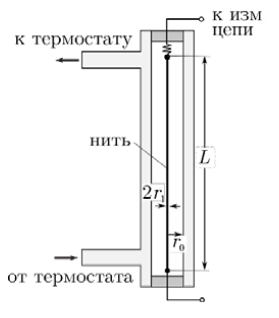
\includegraphics[width=0.3\linewidth]{scheme.png}
		\end{center}
		\caption{Схема установки}
		\label{scheme}
	\end{figure}	
	
	Металлическая нить служит как источником тепла, так и датчиком температуры (термометром сопротивления). По пропускаемому через нить постоянному току I и напряжению U на ней вычисляется мощность нагрева по закону Джоуля–Ленца:
	
	\begin{equation*}
		Q = UI,
	\end{equation*}
	и сопротивление по закону Ома:
	\begin{equation*}
		R = \frac{U}{I}
	\end{equation*}
	
	Сопротивление нити является однозначной функцией её температуры $R(T)$.
	В пределах $20-70 \; ^{\circ} C$ зависимость можно считать линейной $R = R_0 (1 + \alpha(T - T_0))$.
	Эта зависимость может быть получена по данным эксперимента в результате экстраполяции $R(Q)$ при $Q\rightarrow 0$. Иначе, зная материал нити, можно воспользоваться справочными данными.
	
	Для большинства металлов относительное изменение сопротивления из-за нагрева невелико: при изменении температуры на 1 градус относительное изменение сопротивления нити может составлять приблизительно от 0,2 \% до 0,6\% (в зависимости от её материала).
	Следовательно, измерение $R$ важно провести с точностью порядка 0.1\%.
	
	\begin{center}
		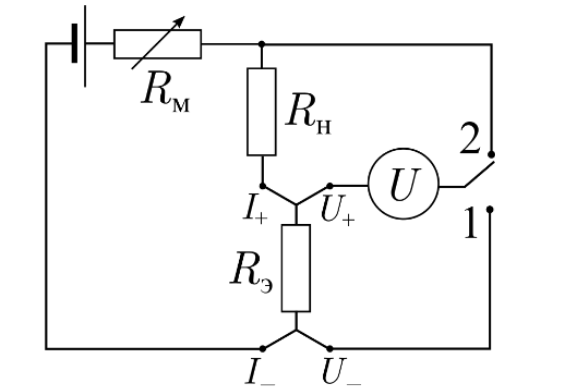
\includegraphics[width=0.5\textwidth]{elec.png}
	\end{center}
	
	На рисунке приведена электрическая схема, используемая в работе.
	
	При фиксированной температуре термостата (и, соответственно, стенок сосуда) будут проведены измерения $U$ и $I$ и получена зависимость $R(Q)$.
	По экстраполяции каждого набора измерений будет найдено $R_0$.
	Таким образом будет получена зависимость $R_0(T)$, из которой будет найден $\alpha$.
	Используя $\alpha = \frac{dR}{dT}$ и $\frac{dQ}{dR}$, получим $\frac{dQ}{d(\Delta T)}$.
	Учитывая уравнение (1) определим коэффициент $\kappa$.
	
	\subsubsection*{Параметры установки}
		$L = (365 \pm 2) \; \text{мм}$ -- длина нити \\
		$2 r_1 = (0.05 \pm 0.005) \; \text{мм}$ -- диаметр нити \\
		Материал нити -- молибден \\
		$2 r_2 = (10 \pm 0.1) \; \text{мм}$ -- диаметр колбы \\
		$R_{\text{э}} = (10.000 \pm 0.001) \; \text{Ом}$ -- эталонное сопротивление \\
		Погрешность вольтметра: $0.0035\% \cdot [\text{измерение}] + 0.0005\% \cdot [\text{предел измерений}]$ \\
		Максимальное напряжение источника: $4 \; \text{В}$
	
	\section*{Ход работы}
	
	$\quad$  Проведем измерения:
	
	\begin{table}[]
		\begin{subtable}{0.4\textwidth}
			\caption*{$T = 22.0 \; ^{\circ} C$}
			\input{UURQ_raw_0.tex}
		\end{subtable}
		\begin{subtable}{0.4\textwidth}
			\caption*{$T = 30.0 \; ^{\circ} C$}
			\input{UURQ_raw_1.tex}
		\end{subtable}
	\hfill
		\begin{subtable}{0.4\textwidth}
			\caption*{$T = 40.0 \; ^{\circ} C$}
			\input{UURQ_raw_2.tex}
		\end{subtable}
		\begin{subtable}{0.4\textwidth}
			\caption*{$T = 50.0 \; ^{\circ} C$}
			\input{UURQ_raw_3.tex}
		\end{subtable}
	\hfill
		\begin{subtable}{0.4\textwidth}
			\caption*{$T = 60.0 \; ^{\circ} C$}
			\input{UURQ_raw_4.tex}
		\end{subtable}
		\begin{subtable}{0.4\textwidth}
			\caption*{$T = 70.0 \; ^{\circ} C$}
			\input{UURQ_raw_5.tex}
		\end{subtable}
	\end{table}

	Погрешности измерений: 
	
	$$\varepsilon(U) = 4 \cdot 10^{-4}  \quad \varepsilon(R_{\text{эт}}) = 1 \cdot 10^{-4} \quad \varepsilon(R) = 6 \cdot 10^{-4} \quad \varepsilon(Q) = 6 \cdot 10^{-4}$$

\newpage
	
	Построим графики $R (Q)$:
	
	\begin{figure}[h]
		\includegraphics{R_Q.pdf}
		\caption{$ \text{Зависимость} \; R(Q)$}
	\end{figure}
	
	По методу наименьших квадратов рассчитаем $R_0$ и $\frac{dR}{dQ}$ и внесем в итоговую таблицу.
	
	Построим график $R_0(T)$:
	
	\begin{figure}[h]
		\includegraphics{R_0_T.pdf}
		\caption{$ \text{Зависимость} \; R_0(T)$}
	\end{figure}
	
	По методу наименьших квадратов рассчитаем $dR/dT$ считая зависимость линейной ($y = ax + b$).
	
	\begin{table}[h]
		\caption{Параметры регрессии $R_0(T)$}
		\begin{tabular}{rrrrrrrrr}
			\toprule
			$\overline{x}$ & $\sigma_x^2$ & $\overline{y}$ & $\sigma_y^2$ & $r_{xy}$ & $a$ & $\Delta a$ & $b$ & $\Delta b$ \\
			\midrule
			4.53e+01 & 2.76e+02 & 15.57 & 5.65e-01 & 1.25e+01 & 0.04528 & 0.00014 & 13.520 & 0.007 \\
			\bottomrule
		\end{tabular}
	\end{table}

	Рассчитаем $\alpha = \frac{1}{R_{273}} \cdot \frac{dR}{dT} = (3.349 \pm 0.011) \cdot 10^{-3} \; 1/\text{K}$ и сравним с табличным значением $\alpha_{\text{табл}} = 4.579 \cdot 10^{-3}$.
	Вероятнее всего в качестве материала нити используется некоторый сплав, который имеет отличную от чистого молибдена.
	
	Приведем итоговую таблицу:

	\begin{table}[h]
		\caption{Итоговая таблица}
		\input{result.tex}
	\end{table}
		
	Построим графики $\kappa (T)$ и $\ln \kappa \; (\ln T)$:
	
	\begin{figure}[H]
		\includegraphics{k_T.pdf}
		\caption{$ \text{Зависимость} \; \kappa (T)$}
	\end{figure}
	
	
	\begin{figure}[H]
		\includegraphics{ln_k_ln_T.pdf}
		\caption{$ \text{Зависимость} \; \ln \kappa \; (\ln T)$}
	\end{figure}
	
	Из $\ln \kappa (\ln T)$ получим $\beta = (0.9 \pm 0.1)$, что плохо согласуется с теоретической оценкой $\beta_{\text{теор}} = 0.5$, предполагающей взаимодействие молекул как упругих шариков
	
	\section*{Вывод}
	
	$\quad$ Метод, используемый в работе, позволяет определить коэффициент теплопроводности воздуха и его зависимость от температуры. Также в работе была получена зависимость сопротивления нити от температуры, что позволяет использовать её в дальнейшем для измерения температуры.
	
	Значение $\beta$ определяется зависимостью $\sigma (T)$, где $\sigma$ -- эффективное сечение столкновений молекул. Значение $\sigma$ убывает с ростом температуры, так как кинетическая энергия начинает преобладать над потенциальной энергией притяжения молекул. Это согласуется с тем, что $\beta > \beta_{\text{теор}}$. 
	
\end{document}